\documentclass[report]{jsbook}
%\documentclass[a4paper]{jsreport}
\RequirePackage[l2tabu, orthodox]{nag}	%古いコマンド,パッケージに対する警告
\usepackage{amsmath, amssymb, amsfonts, amsthm}
\usepackage{ascmac}
\usepackage{bbm}
\usepackage{bigdelim}
\usepackage{cases}
\usepackage{comment}
\usepackage{empheq}
\usepackage{fancybox}
\usepackage{here}
\usepackage{ifthen}
\usepackage{indent}
\usepackage{mathtools}
\usepackage{multirow}
\usepackage{siunitx}
\usepackage{tabularx, arydshln}
\usepackage{udline}
\usepackage{url}
\usepackage[dvipdfmx]{color,graphicx}

\theoremstyle{definition}%定理環境 : 斜体なし
\newtheorem*{commentary}{解説}
\newtheorem*{attention}{注意}
\newtheorem*{solution}{解法}
\newtheorem*{definition}{定義}
\makeatletter
\newcounter{subsubsubsection}
\setcounter{subsubsubsection}{0}
\newcommand{\subsubsubsection}{
	\refstepcounter{subsubsubsection}
	\@startsection{paragraph}{4}{\z@}%
	{1.0\Cvs \@plus.5\Cdp \@minus.2\Cdp}%
	{.1\Cvs \@plus.3\Cdp}%
	{\reset@font\sffamily\normalsize}
}
\makeatother
\setcounter{secnumdepth}{4}

%section, subsection, subsubsection の先頭に部番号が付くようにする
\makeatletter
\@addtoreset{chapter}{part}\renewcommand{\thechapter}{\thepart.\arabic{chapter}}
\@addtoreset{section}{chapter}\renewcommand{\thesection}{\thechapter.\arabic{section}}
\@addtoreset{subsection}{section}\renewcommand{\thesubsection}{\thesection.\arabic{subsection}}
\@addtoreset{subsubsection}{subsection}\renewcommand{\thesubsubsection}{\thesubsection.\arabic{subsubsection}}
\@addtoreset{subsubsubsection}{subsubsection}\renewcommand{\thesubsubsubsection}{\thesubsubsection.\arabic{subsubsubsection}}

\renewcommand{\theequation}{\arabic{equation}}%jsbook によって書き換えられた \theequation を元に戻す

%part, chapter, section, subsection, subsubsection, subsubsubsection 毎に数式,図番号をリセットする
\@addtoreset{equation}{part}
\@addtoreset{equation}{chapter}
\@addtoreset{equation}{section}
\@addtoreset{equation}{subsection}
\@addtoreset{equation}{subsubsection}
\@addtoreset{equation}{subsubsubsection}

\@addtoreset{figure}{part}
\@addtoreset{figure}{chapter}
\@addtoreset{figure}{section}
\@addtoreset{figure}{subsection}
\@addtoreset{figure}{subsubsection}
\@addtoreset{figure}{subsubsubsection}

% @dottedtocline の空白版
\newcommand{\@motchyTocline}[5]{%
	\ifnum #1>\c@tocdepth \else
	\vskip \z@ \@plus.2\p@
	{%
		\leftskip #2\relax \rightskip \@tocrmarg \parfillskip -\rightskip
		\parindent #2\relax\@afterindenttrue
		\interlinepenalty\@M
		\leavevmode
		\@lnumwidth #3\relax
		\advance\leftskip \@lnumwidth \null\nobreak\hskip -\leftskip
		\textbf{\footnotesize #4}\nobreak
		\leaders\hbox{$\m@th \mkern \@dotsep mu\hbox{\quad}\mkern \@dotsep
		mu$}\hfill \nobreak\hb@xt@\@pnumwidth{%
		\hfil\normalfont \normalcolor #5}\par%
	}\fi%
}

%目次の番号とタイトルが重ならないようにする
%dottedtocline{A}{B}{C}のパラメータABC
%	A:目次を生成するレベル(\chapterはレベル0、\sectionはレベル1...)
%	B:一番外側からの左マージン
%	C:見出し番号が入るボックスの幅
\renewcommand{\l@chapter}{\@motchyTocline{0}{0em}{7em}}
\renewcommand{\l@section}{\@dottedtocline{1}{1em}{7em}}
\renewcommand{\l@subsection}{\@dottedtocline{2}{2em}{6em}}
\renewcommand{\l@subsubsection}{\@dottedtocline{3}{3em}{5em}}
\makeatother

\setcounter{tocdepth}{4}%subsubsubsection まで目次に表示する

%% includes MotchyMacros.tex
% for WSL
\input{/mnt/c/Users/motchy/OneDrive/home/individual/motchy/data/hobby/computer/machine-independent/programming/study/languages/LaTex/motchyMacros/motchyMacros}
% for Linux
%\input{/home/motchy/Insync/motchy869@gmail.com/OneDrive/home/individual/motchy/data/hobby/computer/machine-independent/programming/study/languages/LaTex/motchyMacros/motchyMacros}

\begin{document}
	\title{motchyの信号処理備忘録}
	\author{motchy}
	\date{\西暦 2019年11月16日 $\sim$ \today}
	\maketitle
	{\scriptsize \tableofcontents}

	\newcommand{\cycConv}[2]{\underset{\text{cyc}}{{#1}*{#2}}}

	\part{表記法}
	\chapter{数学記号}
		\newcommand*{\uBox}{u_\text{box}}
		\begin{itemize}
			\item $\field$: 体
			\item $\integers$: 整数全体の集合
			\item $\realNumbers$: 実数全体の集合
			\item $\complexNumbers$: 複素数全体の集合
			\item $\bm{x}[i]$:ベクトル $\bm{x}$ の第 $i$ 成分
			\item $\bm{a} \HadamardDiv \bm{b}\;(d \in \naturalNumbers,\;\bm{a},\bm{b} \in \field^d,\;b_i\neq 0 \text{ for all }i)$: $[a_1/b_1,\dots,a_d/b_d]^\top$
			\item $a\%b\;(a,b\in\integers,\;b\neq 0)$: $a$を$b$で割った余り。符号に2通り考えられるが、本書では結果を0以上$|a|$未満とする定義を採用する。
			\item $\bm{a}\%\bm{b}\;(d\in\naturalNumbers,\;\bm{a},\bm{b} \in \integers^d,\; b_i\neq 0 \text{ for all }i)$: $[a_1\%b_1,\dots,a_d\%b_d]^\top$
			\item $\bm{x} \leq \bm{y}\;(d\in\naturalNumbers,\;\bm{x},\bm{y} \in \realNumbers^d) :\Leftrightarrow x_i \leq y_i \text{ for all }i$。$\geq, <, >$についても同様。
			\item $\uBox$: 単位矩形関数。区間 $[-1/2,1/2]$ に属する数を 1 に移し、それ以外の数を 0 に移す。
		\end{itemize}
	\chapter{量の次元の扱い}
		本書では数学との整合性と普遍性を重視して写像の引数は全て無次元量とし、座標や時間も無次元量とする。
		本書で述べられる定理は量の次元や計量単位に依存せず、応用し易い。
		\par
		しかし、記号に量の次元を含めない姿勢を実用の場で徹底するのは難しい。
		例えば何らかの開発プロジェクトに於いては、記号に次元を含めておく方が説明が簡便になるし、次元解析にも役立つ。
		量の次元と数学との整合性を保つ現実的な方針は次のようであろう。
		\begin{itemize}
			\item 物理量を表す記号には必ず量の次元を含める
			\item 写像の引数は必ず無次元量とする
			\item 量の次元をもつ量を写像の引数の位置に‘書く’ときは、その量を計量単位で除した数を引数と‘する’ものと約束する。
		\end{itemize}
	\chapter{連続座標信号の表現}
		連続的な座標値$\bm{x}\in\realNumbers^{d_1}\;(d_1\in\naturalNumbers)$から$\realNumbers^{d_2}\;(d_2\in\naturalNumbers)$への写像を$d_1$次元連続座標信号という。
		信号値は全ての座標に対して定義される必要はない。
		\par
		例えばカセットテープレコーダーに記録された音声信号は$d_1=d_2=1$のものである。
		\par
		信号$f$の位置$\bm{x} = [x_1,x_2,\dots,x_{d_1}]^\top$での値を$f(\bm{x})$や$f(x_1,\dots,x_{d_1})$で表す。
	\chapter{離散座標信号の表現}
		離散的な座標値$\bm{x}\in\integers^{d_1}\;(d_1\in\naturalNumbers)$から$\realNumbers^{d_2}\;(d_2\in\naturalNumbers)$への写像を$d_1$次元離散座標信号という。
		信号値は全ての座標に対して定義される必要はない。
		\par
		例えば離散的な時刻での電圧のサンプリングデータは$d_1=d_2=1$のものである(この場合の「座標」は時間軸上での座標という意味になる)。
		また、コンピュータのディスプレイに映る2次元カラー画像は$d_1=2,d_2=3$のものである。
		\par
		信号$f$の位置$\bm{x} = [x_1,x_2,\dots,x_{d_1}]^\top$での値を$f(\bm{x})$や$f(x_1,\dots,x_{d_1})$で表す。

	\part{畳み込み}
	\chapter{畳み込みの微分}
		\section{関係式}
			\begin{shadebox}
				微分可能な複素数値信号 $x_1, x_2:\realNumbers\to\complexNumbers$ に畳み込みが存在するとき、次が成り立つ。
				\[ \derivLong{(x_1*x_2)(t)}{t}{} = {x_1}'*x_2 = x_1*{x_2}' \]
			\end{shadebox}
			\begin{proof}
				\quad\par
				まず次式が成り立つ。
				\begin{align*}
					\derivLong{(x_1*x_2)(t)}{t}{} &= \derivLong{\integrate{-\infty}{\infty}{x_1(\tau)x_2(t-\tau)}{}{\tau}}{t}{} = \integrate{-\infty}{\infty}{x_1(\tau)\derivLong{x_2(t-\tau)}{t}{}}{}{\tau} \\
					&= \integrate{-\infty}{\infty}{x_1(\tau){x_2}'(t-\tau)}{}{\tau} = (x_1*{x_2}')(t)
				\end{align*}
				$x_1*x_2 = x_2*x_1$ を用いて上記と同様の計算を行うと次式が成り立つ。
				\[ \derivLong{(x_1*x_2)(t)}{t}{} = ({x_1}'*x_2)(t) \]
			\end{proof}
		\section{使いどころ}
			例えばディジタル信号処理で役立つときがある。
			前記の関係式の離散座標版も同様に成り立つ。
			(a) 長い入力信号に(b) (それに比べて短い)時間的に変化しない信号(典型的には FIR フィルタの係数)を畳み込むとき、後者の時間微分(典型的には差分で近似)を予め計算しておいて (a) と畳み込めば、微分のオンライン計算が不要になる。
	\chapter{巡回畳み込み}
		\label{巡回畳み込み}
		$\Omega \coloneq \{0,1,\dots,N_1-1\}\times\{0,1,\dots,N_2-1\}\times\cdots\times\{0,1,\dots,N_d-1\}$とする。
		$f,g$を周期が$(N_1,\dots,N_d)$であるような離散座標信号$f,g: \Omega\to\complexNumbers;\;\bm{n} = [n_1,n_2,\dots,n_d]^\top \mapsto f(\bm{n}),g(\bm{n})$とする。
		$\bm{N} \coloneq [N_1,\dots,N_d]^\top$とする。
		$f$と$g$の巡回畳み込み$\cycConv{f}{g}$を次式で定義する。
		\[ \left(\cycConv{f}{g}\right)(\bm{n}) \coloneq \sum_{\bm{m} \in\Omega} f(\bm{m})g((\bm{n}-\bm{m})\%\bm{N}) \]

		\section{巡回畳み込みの可換則}
			\begin{shadebox}
				$\Omega,f,g$の定義を\ref{巡回畳み込み}と同じものとするとき、次が成り立つ。
				\[ \cycConv{f}{g} = \cycConv{g}{f} \]
			\end{shadebox}
			\begin{proof}
				\begin{align}
					\left(\cycConv{g}{f}\right)(\bm{n}) &= \sum_{\bm{m}\in\Omega} g(\bm{m})f((\bm{n}-\bm{m})\%\bm{N}) \nonumber \\
					&= \sum_{m_1=0}^{N_1-1}\sum_{\bm{m}_2\in\Omega_2}g(m_1,\bm{m}_2)f((n_1 - m_1)\%N_1,(\bm{n_2}-\bm{m_2})\%\bm{N_2})
				\end{align}
				ここに$\bm{n}_i \coloneq [n_i,\dots,n_d]^\top\;(\bm{m}_i,\bm{N}_i\text{も同様}),\;\Omega_i \coloneq \{0,1,\dots,N_i-1\}\times\cdots\times\{0,1,\dots,N_d-1\}$である。
				\begin{align*}
					(1) &= \sum_{m_1=0}^{n_1}\sum_{\bm{m}_2\in\Omega_2}g(m_1,\bm{m}_2)f(n_1 - m_1,(\bm{n_2}-\bm{m_2})\%\bm{N_2}) \\
					&\quad + \sum_{m_1=n_1+1}^{N_1-1}\sum_{\bm{m}_2\in\Omega_2}g(m_1,\bm{m}_2)f(n_1 + N_1 - m_1,(\bm{n_2}-\bm{m_2})\%\bm{N_2}) \\
					&= \sum_{l_1=n_1}^0 \sum_{\bm{m}_2\in\Omega_2}g(n_1 - l_1,\bm{m}_2)f(l_1,(\bm{n_2}-\bm{m_2})\%\bm{N_2}) \\
					&\quad + \sum_{l_1=N_1-1}^{n_1+1}\sum_{\bm{m}_2\in\Omega_2}g(n_1+N_1-l_1,\bm{m}_2)f(l_1,(\bm{n_2}-\bm{m_2})\%\bm{N_2}) \\
					&= \sum_{l_1=n_1}^0 \sum_{\bm{m}_2\in\Omega_2}g(\textcolor{darkpastelgreen}{(n_1-l_1)\%N_1},\bm{m}_2)f(l_1,(\bm{n_2}-\bm{m_2})\%\bm{N_2}) \\
					&\quad + \sum_{l_1=N_1-1}^{n_1+1}\sum_{\bm{m}_2\in\Omega_2}g((n_1-l_1)\%N_1,\bm{m}_2)f(l_1,(\bm{n_2}-\bm{m_2})\%\bm{N_2}) \\
					&= \sum_{l_1=0}^{N_1-1} \sum_{\bm{m}_2\in\Omega_2}g((n_1-l_1)\%N_1,\bm{m}_2)f(l_1,(\bm{n_2}-\bm{m_2})\%\bm{N_2}) \\
				\end{align*}
				同様の変形を繰り返すと最終的に次のようになる。
				\[ \left(\cycConv{g}{f}\right)(\bm{n}) = \sum_{\bm{l}\in\Omega} g((\bm{n}-\bm{l})\%\bm{N})f(\bm{l}) = \left(\cycConv{f}{g}\right)(\bm{n}) \]
			\end{proof}
		\chapter{諸定理}
			\section{線形変換と畳み込みの順序交換}
				\subsection{動機}
					画像処理に於いてカーネルとの畳み込みを実行してから線形変換を施す場合と、事前に画像とカーネルの両方に線形変換を施してから畳み込む場合の結果の違いに関心がある。
				\subsection{理論}
					$d\in\naturalNumbers$とし、$f:\bm{x}\in\realNumbers^d\mapsto f(\bm{x})\in\realNumbers$を$d$次元信号とする。
					線形変換を表す正則行列を$A$とし、$A$による変換を$T_A$と表す。
					$T_A$による変換は次式を以て定義する。
					\[ T_A(f)(\bm{x}) = f(A^{-1}\bm{x}) \]
					$G:\bm{x}\in\realNumbers^d\mapsto G(\bm{x})\in\realNumbers$を$d$次元信号とする。
					このとき次式が成り立つ。
					\[ T_A(G)*T_A(f) = |A|T_A(G*f) \]
					\begin{proof}
						\quad\par
						$\mu$をJordan測度とする。
						\begin{align*}
							T_A(G)*T_A(f)(\bm{x}) &= \LebInteg{\realNumbers^d}{T_A(G)(\bm{x}-\bm{u})T_A(f)(\bm{u})}{\mu}{\bm{u}} = \LebInteg{\realNumbers^d}{G(A^{-1}(\bm{x}-\bm{u}))f(A^{-1}\bm{u})}{\mu}{\bm{u}} \\
							&= \LebInteg{\realNumbers^d}{G(A^{-1}\bm{x} - A^{-1}\bm{u})f(A^{-1}\bm{u})}{\mu}{\bm{u}} \\
							&= \LebInteg{\realNumbers^d}{G(A^{-1}\bm{x} - \bm{v})f(\bm{v})}{\abs{|A|}\mu}{\bm{v}} \\
							&\phantom{=} (\bm{v}=A^{-1}\bm{u}\text{と変数変換した。}\abs{|A|}\text{は}|A|の絶対値である。) \\
							&= \abs{|A|} \LebInteg{\realNumbers^d}{G(A^{-1}\bm{x} - \bm{v})f(\bm{v})}{\mu}{\bm{v}} \\
							&= \abs{|A|}T_A(G*f)(\bm{x})
						\end{align*}
					\end{proof}
				\section{数値実験}
					Mathematicaによる例が「線形変換と畳み込み.nb」にある。
	\part{Fourier解析}
		\chapter{Fourier級数展開}
			\section{基底関数}
				Fourier級数展開の基底関数はFourier変換やDFTのものと違って正規化されていないため、美しさに欠ける。
				\par
				$d\in\naturalNumbers,\;W_l>0\;(l=1,2,,\cdots,d),\;\bm{k}\in\integers^d$とする。
				次式で定義される、$\bm{x}\in\realNumbers^d$に関する連続座標信号を、区間$\prod_{l=1}^d [-W_l,W_l]$に於ける第$\bm{k}$基底関数という。
				\[ W(\bm{k},\bm{x}) \coloneqq \exp i\sum_{l=1}^d k_l\frac{x_l}{W_l}\pi \]

			\section{Fourier係数}
				$d\in\naturalNumbers,\;W_l>0\;(l=1,2,,\cdots,d),\;\Omega\coloneqq\prod_{l=1}^d [-W_l,W_l],\;\bm{k}\in\integers^d$とする。
				$f:\bm{x}\in\realNumbers \mapsto f(\bm{x})\in\realNumbers$を、第$l$座標に関して周期が$2W_l$であるような周期関数とする。
				次式で定義する、$\bm{k}$に関する離散座標信号を$f$の第$\bm{k}$ Fourier係数という。
				\[ c(f,\bm{k}) \coloneqq \left(\prod_{l=1}^d 2W_l\right)^{-1}\integrate{\Omega}{}{\conj{W(\bm{k},\bm{x})}f(\bm{x})}{}{\bm{x}} \]

		\chapter{Fourier変換}
			\section{基底関数}
				$d\in\naturalNumbers,\;\bm{x},\bm{\omega}\in\realNumbers^d$とする。
				次のものを$d$次元Fourier変換に於ける基底関数という。
				\[ W(\bm{\omega},\bm{x}) \coloneqq (2\pi)^{-d/2}\exp i\bm{\omega}^\top\bm{x} \]

			\section{Fourier変換の定義}
				$d\in\naturalNumbers,\;\bm{\omega}\in\realNumbers^d$とする。
				$f:\realNumbers^d\to\complexNumbers$に対して、次式で定義される、$\bm{\omega}$に関する連続座標信号を$f$のFourier変換という。
				\[ \mathcal{F}(f,\bm{\omega}) \coloneqq \integrate{\realNumbers^d}{}{\conj{W(\bm{\omega},\bm{x})}f(\bm{x})}{}{\bm{x}} = (2\pi)^{-d/2} \integrate{\realNumbers^d}{}{\exp (-i\bm{\omega}^\top\bm{x})f(\bm{x})}{}{\bm{x}} \]

		\chapter{離散時間Fourier変換(DTFT)}
			\section{直観的な説明}
				離散時間Fourier変換(Discrete Time Fourier Transform; DTFT)とは、直観的には、離散座標信号を、連続的な周波数をもつ無数の離散時間信号の重ね合わせとして表現するものである。
			\section{定義}
				$d\in\naturalNumbers,\;\bm{T}_\text{s}(\in\realNumbers^d)>\bm{0}$とする。
				$f:\integers^d\to\complexNumbers$に対して、次式で定義される、$\bm{\omega}\in\realNumbers^d$に関する連続座標信号を$f$の離散時間Fourier変換という。
				\[ \text{DTFT}(f,\bm{\omega}) \coloneqq \sum_{\bm{n}\in\integers^d} f(\bm{n})\exp(-i(\bm{\omega}\HadamardProd\bm{T}_\text{s})^\top\bm{n}) \]
				$\bm{\omega}$は各軸方向の角周波数をまとめて表したベクトルであり、$\bm{T}_\text{s}$は各軸方向のサンプリング周期である。
				DTFTは$\bm{\omega}$に関する周期関数であり、その周期は$2\pi\bm{1}\HadamardDiv\bm{T}_\text{s}$である。
				\subsection{呼称について}
					本書では関数の引数を時間や周波数に限定せず、より一般に座標と呼ぶ姿勢をとっている。
					しかしDTFTは電気・電子系の信号処理の分野で発展したため、離散``時間''という呼称が浸透しており、これに敢えて逆らって離散``座標''と呼ぶのは本書と工学応用の相性を悪くするだけで無益である。
					そこで、DTFTのような、歴史的な理由で呼称が定着しているものについては慣例に従うことにする。
			\section{連続座標信号との関係}
				連続座標信号$f_\text{c}:\realNumbers^d\to\complexNumbers$をサンプリング周期$\bm{T}_\text{s} \coloneqq [T_{\text{s},1}, T_{\text{s},2}, \dotsc, T_{\text{s},d}]^\top\in\realNumbers^d$すなわち周波数$\bm{f}_\text{s} \coloneqq [f_{\text{s},1}, f_{\text{s},2}, \dotsc, f_{\text{s},d}]^\top \coloneqq [1/T_{\text{s},1}, 1/T_{\text{s},2}, \dotsc, 1/T_{\text{s},d}]^\top\in\realNumbers^d$でサンプリングした離散座標信号を$f_\text{d}: \bm{n}\in\integers^d\mapsto f_\text{c}(\bm{T}^\top\bm{n})$とする。
				$f_\text{d}$のDTFTに於ける多次元の角周波数$\bm{\omega}$を周波数$\bm{f}$を用いて$\bm{\omega} \coloneqq 2\pi\bm{f}$と表す。
				\par
				$\bm{n}$の第$k$要素$n_k$が1だけ変化すると、元の連続座標信号の対応する座標は$T_k$だけ変化し、DTFTのカーネル関数$\exp(i(\bm{\omega}\HadamardProd\bm{T}_\text{s})^\top\bm{n})$の偏角は$\omega_k T_{\text{s},k} = 2\pi f_k T_{\text{s},k}$だけ変化する。
				つまりDTFTの定義域に於ける周波数$\bm{f}$の第$k$成分に対応する元の連続座標信号の周波数の第$k$成分は$f_k$であり、スケールは保たれている。
				\par
				DTFTの定義で述べたように、DTFTは周期が$2\pi\bm{1}\HadamardDiv\bm{T}_\text{s}$であるから、一意に区別できる角周波数は$-\bm{\pi}\HadamardDiv\bm{T}_\text{s} \leq \bm{\omega} < \bm{\pi}\HadamardDiv\bm{T}_\text{s}$、つまり一意に区別できる周波数は$-\bm{f}_\text{s}/2 \leq \bm{f} < \bm{f}_\text{s}/2$である。
				この事実と、先程述べたDTFTと元の連続座標信号との周波数の関係から、DTFTに於いて一意に区別できる周波数に対応する元の連続座標信号の周波数$\tilde{\bm{f}}$は$-\bm{f}_\text{s}/2 \leq \tilde{\bm{f}} < \bm{f}_\text{s}/2$である。
			\section{逆離散時間Fourier変換(IDTFT)}
				$d\in\naturalNumbers,\;\bm{T}_\text{s}(\in\realNumbers^d)>\bm{0},\;\Omega := \prod_{k=1}^d [-\pi/T_{\text{s},k},\pi/T_{\text{s},k})$とする。
				$F:\realNumbers^d\to\complexNumbers$に対して、次式で定義される、$\bm{n}\in\integers^d$に関する離散座標信号を$F$の逆離散時間Fourier変換(Inverse DTFT; IDTFT)という。
				\[ \text{IDTFT}(F,\bm{n}) \coloneqq \frac{\prod_{k=1}^d T_{\text{s},k}}{(2\pi)^d}\integrate{\Omega}{}{F(\bm{\omega})\exp(i(\bm{\omega}\HadamardProd\bm{T}_\text{s})^\top\bm{n})}{}{\bm{\omega}} \]
				\subsection{IDTFTがDTFTの逆変換であること}
					厳密な導出はここでは述べないが、$\sum_{\bm{n}\in\integers^d} f(\bm{n})$が絶対収束する場合は$\text{IDTFT}(\text{DTFT}(f,\bm{\omega}),\bm{n}) = f(\bm{n})$となることを簡単に証明できる。
					$\sum$と$\int$の順序交換が簡単に行えるからである。
			\section{積と畳み込みとの関係}
				以下では既出の記号の定義は上書きしない限り引き継ぐ。
				$f,g:\integers^d\to\complexNumbers$に対してそのDTFTを$F(\bm{\omega}),G(\bm{\omega})$とする。
				\subsection{時間領域, 周波数領域の畳み込みの定義}
					時間領域の畳み込みを次で定義する:
					\par
					$f,g:\integers^d\to\complexNumbers$に対してその畳み込み$f*g$を次式で定義する。
					\[ (f*g)(\bm{n}) := \sum_{\bm{m}\in\integers^d} f(\bm{m})g(\bm{n}-\bm{m}) \]
					周波数領域の畳み込みを次で定義する:
					\par
					$F,G:\realNumbers^d\to\complexNumbers$に対してその畳み込み$F*G$を次式で定義する。
					\[ (F*G)(\bm{\omega}) := \frac{\prod_{k=1}^d T_{\text{s},k}}{(2\pi)^d}\integrate{\Omega}{}{F(\tilde{\bm{\omega}})G(\bm{\omega}-\tilde{\bm{\omega}})}{}{\tilde{\bm{\omega}}} \]
				\subsection{積のDTFT}
					$f,g$の積のDTFTは次式で求まる。
					\begin{align*}
						\text{DTFT}(fg,\bm{\omega}) &= \sum_{\bm{n}\in\integers^d} f(\bm{n})g(\bm{n})\exp(-i(\bm{\omega}\HadamardProd\bm{T}_\text{s})^\top\bm{n}) = \sum_{\bm{n}\in\integers^d} \text{IDTFT}(F,\bm{n}) g(\bm{n})\exp(-i(\bm{\omega}\HadamardProd\bm{T}_\text{s})^\top\bm{n}) \\
						&= \sum_{\bm{n}\in\integers^d} \left(\frac{\prod_{k=1}^d T_{\text{s},k}}{(2\pi)^d}\integrate{\Omega}{}{F(\tilde{\bm{\omega}})e^{i(\tilde{\bm{\omega}}\HadamardProd\bm{T}_\text{s})^\top\bm{n}}}{}{\tilde{\bm{\omega}}}\right) g(\bm{n})\exp(-i(\bm{\omega}\HadamardProd\bm{T}_\text{s})^\top\bm{n}) \\
						&= \frac{\prod_{k=1}^d T_{\text{s},k}}{(2\pi)^d}\integrate{\Omega}{}{F(\tilde{\bm{\omega}})\left(\sum_{\bm{n}\in\integers^d} g(\bm{n})e^{-i\left((\bm{\omega}-\tilde{\bm{\omega}})\HadamardProd\bm{T}_\text{s}\right)^\top\bm{n}}\right)}{}{\tilde{\bm{\omega}}} \\
						&= \frac{\prod_{k=1}^d T_{\text{s},k}}{(2\pi)^d}\integrate{\Omega}{}{F(\tilde{\bm{\omega}})G(\bm{\omega}-\tilde{\bm{\omega}})}{}{\tilde{\bm{\omega}}} = (F*G)(\omega)
					\end{align*}
				\subsection{畳み込みのDTFT}
					$f,g$の畳み込みのDTFTは次式で求まる。
					\begin{align*}
						\text{DTFT}(f*g,\bm{\omega}) &= \sum_{\bm{n}\in\integers^d} \sum_{\bm{m}\in\integers^d}f(\bm{m})g(\bm{n}-\bm{m})\exp(-i(\bm{\omega}\HadamardProd\bm{T}_\text{s})^\top\bm{n}) \\
						&= \sum_{\bm{m}\in\integers^d} f(\bm{m})\exp(-i(\bm{\omega}\HadamardProd\bm{T}_\text{s})^\top\bm{m}) \sum_{\bm{n}\in\integers^d} g(\bm{n}-\bm{m})\exp(-i(\bm{\omega}\HadamardProd\bm{T}_\text{s})^\top(\bm{n}-\bm{m})) \\
						&= F(\bm{\omega})G(\bm{\omega})
					\end{align*}
				\subsection{積のIDTFT}
					DTFTの可逆性から直ちに言えるが、敢えて直接計算してみる。
					\begin{align*}
						\text{IDTFT}(FG,\bm{n}) &= \frac{\prod_{k=1}^d T_{\text{s},k}}{(2\pi)^d}\integrate{\Omega}{}{F(\bm{\omega})G(\bm{\omega})\exp(i(\bm{\omega}\HadamardProd\bm{T}_\text{s})^\top\bm{n})}{}{\bm{\omega}} \\
						&= \frac{\prod_{k=1}^d T_{\text{s},k}}{(2\pi)^d}\integrate{\Omega}{}{\left(\text{DTFT}(f,\bm{\omega})\right)G(\bm{\omega})\exp(i(\bm{\omega}\HadamardProd\bm{T}_\text{s})^\top\bm{n})}{}{\bm{\omega}} \\
						&= \frac{\prod_{k=1}^d T_{\text{s},k}}{(2\pi)^d}\integrate{\Omega}{}{\left(\sum_{\bm{m}\in\integers^d} f(\bm{m})\exp(-i(\bm{\omega}\HadamardProd\bm{T}_\text{s})^\top\bm{m})\right)G(\bm{\omega})\exp(i(\bm{\omega}\HadamardProd\bm{T}_\text{s})^\top\bm{n})}{}{\bm{\omega}} \\
						&= \sum_{\bm{m}\in\integers^d} f(\bm{m}) \frac{\prod_{k=1}^d T_{\text{s},k}}{(2\pi)^d} \integrate{\Omega}{}{G(\bm{\omega})\exp(i(\bm{\omega}\HadamardProd\bm{T}_\text{s})^\top(\bm{n}-\bm{m}))}{}{\bm{\omega}} \\
						&= \sum_{\bm{m}\in\integers^d} f(\bm{m})g(\bm{n}-\bm{m}) = (f*g)(\bm{n})
					\end{align*}
				\subsection{畳み込みのIDTFT}
					DTFTの可逆性から直ちに言えるが、敢えて直接計算してみる。
					\begin{align*}
						&\phantom{=} \text{IDTFT}(F*G,\bm{n}) \\
						&= \frac{\prod_{k=1}^d T_{\text{s},k}}{(2\pi)^d}\integrate{\bm{\omega}\in\Omega}{}{(F*G)(\bm{\omega})\exp(i(\bm{\omega}\HadamardProd\bm{T}_\text{s})^\top\bm{n})}{}{\bm{\omega}} \\
						&= \frac{\prod_{k=1}^d T_{\text{s},k}}{(2\pi)^d}\integrate{\bm{\omega}\in\Omega}{}{\left(\frac{\prod_{k=1}^d T_{\text{s},k}}{(2\pi)^d}\integrate{\tilde{\bm{\omega}}\in\Omega}{}{F(\tilde{\bm{\omega}})G(\bm{\omega}-\tilde{\bm{\omega}})}{}{\tilde{\bm{\omega}}}\right)\exp(i(\bm{\omega}\HadamardProd\bm{T}_\text{s})^\top\bm{n})}{}{\bm{\omega}} \\
						&=
						\frac{\prod_{k=1}^d T_{\text{s},k}}{(2\pi)^d} \int_{\tilde{\bm{\omega}}\in\Omega} \left(\frac{\prod_{k=1}^d T_{\text{s},k}}{(2\pi)^d}\integrate{\bm{\omega}\in\Omega}{}{G(\bm{\omega}-\tilde{\bm{\omega}})\exp(i((\bm{\omega}-\tilde{\bm{\omega}})\HadamardProd\bm{T}_\text{s})^\top\bm{n})}{}{\bm{\omega}}\right) \\
						&\phantom{=} F(\tilde{\bm{\omega}})\exp(i(\tilde{\bm{\omega}}\HadamardProd\bm{T}_\text{s})^\top\bm{n})\mathrm{d}\bm{\tilde{\bm{\omega}}} \\
						&= \frac{\prod_{k=1}^d T_{\text{s},k}}{(2\pi)^d}\integrate{\tilde{\bm{\omega}}\in\Omega}{}{g(\bm{n})F(\tilde{\bm{\omega}})\exp(i(\tilde{\bm{\omega}}\HadamardProd\bm{T}_\text{s})^\top\bm{n})}{}{\tilde{\bm{\omega}}} \\
						&= f(\bm{n})g(\bm{n})
					\end{align*}
			\section{定数関数1のDTFT}
				\label{定数関数1のDTFT}
				簡単のため1次元の場合について考察する。
				工学系の学生を対象とする講義では、$\text{DTFT}(1,\omega) = (2\pi/T_\text{s})\sum_{m\in\integers}\delta(\omega-2m\pi/T_\text{s})$($\delta$はDiracのデルタ関数)を詳細を割愛して結果として受け入れさせる場合が多いと思う。
				$\text{IDTFT}\left((2\pi/T_\text{s})\sum_{m\in\integers}\delta(\omega-2m\pi/T_\text{s}),x\right)=1$の確認は簡単であり、DTFTの可逆性から$\text{DTFT}(1,\omega) = (2\pi/T_\text{s})\sum_{m\in\integers}\delta(\omega-2m\pi/T_\text{s})$を受け入れる説明がなされると思う。
				\par
				ここではDirichlet積分を用いて$\text{DTFT}(1,\omega) = (2\pi/T_\text{s})\sum_{m\in\integers}\delta(\omega-2m\pi/T_\text{s})$を直接的に導出してみる。
				DTFTの定義から次式が成り立つ。
				\[
					\text{DTFT}(1,\omega) = \lim_{N\to\infty} \sum_{m=-N}^N e^{i\omega T_\text{s} m} = \frac{\sin(N+1/2)\omega T_\text{s}}{\sin(\omega T_\text{s}/2)}
				\]
				最右辺は等比数列の和の公式を用いた後、分母と分子に$e^{-i\omega/2}$を掛けて整理すると得られる。
				これが$N\to\infty$で$(2\pi/T_\text{s})\sum_{m\in\integers}\delta(\omega-2m\pi/T_\text{s})$として振る舞うことを確かめる。
				$2\pi/T_\text{s}$周期性については明らかだから、$[-\pi/T_\text{s},\pi/T_\text{s})$の範囲で$(2\pi/T_\text{s})\delta(\omega)$として振る舞うことを確かめれば十分である。
				示すべきことは次の通りである。
				\begin{shadebox}
					$d\in\naturalNumbers$とする。
					区間$\Omega \subseteq [-\pi/T_\text{s},\pi/T_\text{s})$上で連続な任意の関数$f:\Omega\to\complexNumbers^d$を考える。
					$h>0$を$[-h,h) \subseteq \Omega$となるように任意にとる。
					このとき次式が成り立つ。
					\[
						\lim_{N\to\infty} \integrate{-h}{h}{\frac{\sin(N+1/2)x T_\text{s}}{\sin(x T_\text{s}/2)} f(x)}{}{x} = \frac{2\pi}{T_\text{s}} f(0)
					\]
				\end{shadebox}
				\begin{proof}
					\quad\par
					極限をとる前の積分を$I_N$とおく。
					$y = x T_\text{s}/2$と変数変換すると次式を得る。
					\[
						I_N = \frac{2}{T_\text{s}}\integrate{-h T_\text{s}/2}{h T_\text{s}/2}{\frac{\sin(2N+1)y}{\sin y}f(2y/T_\text{s})}{}{y} = \frac{2}{T_\text{s}}\integrate{-h T_\text{s}/2}{h T_\text{s}/2}{\frac{\sin(2N+1)y}{y}\frac{y}{\sin y}f(2y)}{}{y}
					\]
					後に現れるDirichlet積分の性質から$N\to\infty$で積分の主要部分が$x=0$近傍に集中することがこの時点で推察できる。
					そこで、十分に小さい正数$d'$を$0<d'<h T_\text{s}/2$となるようにとり、積分区間を$[-h T_\text{s}/2,-d']\cup[-d',d']\cup[d',h T_\text{s}/2]$と分割する。
					\par
					$[-h T_\text{s}/2,-d'], [d',h T_\text{s}/2]$に於いて$f(2y/T_\text{s})/\sin y$は一様連続であるので$N\to\infty$でこの2つの区間に於ける$(f(2y/T_\text{s})\sin(2N+1)y)/\sin y$の積分は0に収束する。
					証明の方針としては、$\sin(2N+1)y$の符号が変化する点で積分区間を細分し、各区間内で$f(2y/T_\text{s})/\sin y$を定数で近似して全体の積分を近似すると、一様連続性から近似値と真の積分の差が0に収束し、かつ近似値が0に収束する。
					\par
					つまり任意に小さい$\varepsilon>0$に対して、$d'$に依存して決まる十分大きい自然数$N_1$が存在して次式が成り立つ。
					\[
						N\geq N_1 \Rightarrow \abs{\frac{2}{T_\text{s}}\integrate{[-h T_\text{s}/2,-d']\cup[d',h T_\text{s}/2]}{}{\frac{\sin(2N+1)y}{\sin y}f(2y/T_\text{s})}{}{y}}<\varepsilon
					\]
					\par
					次に$[-d',d']$に於ける積分を評価する。
					$y\to 0$で$y/\sin y\to 1,\;f(2y/T_\text{s})\to f(0)$であるから、$d'$を十分小さくとりなおすことで$|f(2y/T_\text{s})y/\sin y - f(0)| < \varepsilon$となり次式が成り立つ。
					\[
						\abs{\frac{2}{T_\text{s}}\integrate{-d'}{d'}{\frac{\sin(2N+1)y}{y}\frac{y}{\sin y}f(2y/T_\text{s})}{}{y} - \frac{2}{T_\text{s}}f(0)\integrate{-d'}{d'}{\frac{\sin(2N+1)y}{y}}{}{y}} < \frac{2\varepsilon}{T_\text{s}}\abs{\integrate{-d'}{d'}{\frac{\sin(2N+1)y}{y}}{}{y}}
					\]
					最後にDirichlet積分を用いて$(\sin(2N+1)y)/\sin y$の積分を評価する。
					\[
						\integrate{-d'}{d'}{\frac{\sin(2N+1)y}{y}}{}{y} = 2\integrate{0}{d'}{\frac{\sin(2N+1)y}{y}}{}{y} = 2\integrate{0}{(2n+1)d'}{\frac{\sin z}{z}}{}{z} \to \pi \text{ as } n\to\infty
					\]
					すなわち$d'$に依存して決まる十分大きい自然数$N_2$が存在して次式が成り立つ。
					\[ N\geq N_1 \Rightarrow \abs{\integrate{-d'}{d'}{\frac{\sin(2N+1)y}{y}}{}{y} - \pi} < \varepsilon \]
					以上より、$d'>0$を十分に小さくとり、$N\geq\max(N_1,N_2)$とすれば次式が成り立つ。
					\begin{align*}
						\abs{I_N - \frac{2\pi}{T_\text{s}} f(0)} &= \left|\underbrace{\left(\frac{2}{T_\text{s}}f(0)\integrate{-d'}{d'}{\frac{\sin(2N+1)y}{y}}{}{y} - \frac{2\pi}{T_\text{s}} f(0)\right)}_{(1)} \right. \\
						&\phantom{=} \left.+ \underbrace{\left(\frac{2}{T_\text{s}}\integrate{-d'}{d'}{\frac{\sin(2N+1)y}{y}\frac{y}{\sin y}f(2y)}{}{y} - \frac{2}{T_\text{s}}f(0)\integrate{-d'}{d'}{\frac{\sin(2N+1)y}{y}}{}{y}\right)}_{(2)} \right. \\
						&\phantom{=} \left.+ \underbrace{\frac{2}{T_\text{s}}\integrate{[-h/2,-d']\cup[d',h/2]}{}{\frac{\sin(2N+1)y}{\sin y}f(2y)}{}{y}}_{(3)}\right| \\
						&\leq |(1)| + |(2)| + |(3)| < \frac{2f(0)}{T_\text{s}}\varepsilon + \frac{2\varepsilon}{T_\text{s}}(\pi+\varepsilon) + \varepsilon
					\end{align*}
				\end{proof}
			\section{単一周波数波のDTFTの導出}
				\newcommand{\Ts}{T_\text{s}}
				$T_\text{s}>0$とする。
				$\sin(\omega_0 T_\text{s} n + \phi)\;(\omega_0\in\realNumbers, n\in\integers)$のDTFTは\ref{定数関数1のDTFT}の結果を用いて次のようにして得られる。
				\begin{align*}
					\text{DTFT}(\sin(\omega_0 T_\text{s} n + \phi), \omega) &= \frac{1}{2i}\sum_{m\in\integers} \bigl(\exp(i(\omega_0\Ts m + \phi) - \exp(-i(\omega_0\Ts m + \phi))\bigr)\exp(-i\omega\Ts m) \\
					&= \frac{1}{2i}\sum_{m\in\integers} \left(e^{i\phi}\exp(i(\omega_0-\omega)\Ts m) - e^{-i\phi}\exp(i(-\omega_0-\omega)\Ts m)\right) \\
					&= \frac{1}{2i}e^{i\phi}\sum_{m\in\integers}\delta(\omega_0-\omega - 2\pi m/\Ts) - \frac{1}{2i}e^{-i\phi}\sum_{m\in\integers}\delta(-\omega_0-\omega - 2\pi m/\Ts) \\
					&= \frac{1}{2i}e^{i\phi}\sum_{m\in\integers}\delta(-(\omega-\omega_0) - 2\pi m/\Ts) - \frac{1}{2i}e^{-i\phi}\sum_{m\in\integers}\delta(-(\omega+\omega_0) - 2\pi m/\Ts) \\
					&= \frac{1}{2i}e^{i\phi}\frac{2\pi}{\Ts}\sum_{m\in\integers}\delta(\omega-\omega_0 - 2\pi m/\Ts) - \frac{1}{2i}e^{-i\phi}\frac{2\pi}{\Ts}\sum_{m\in\integers}\delta(\omega+\omega_0 - 2\pi m/\Ts) \\
					&= \frac{\pi}{\Ts i}\sum_{m\in\integers}\left(e^{i\phi}\delta(\omega-\omega_0 - 2\pi m/\Ts) - e^{-i\phi}\delta(\omega+\omega_0 - 2\pi m/\Ts)\right)
				\end{align*}
				上の結果を利用して、$\cos(\omega_0 T_\text{s} n + \phi)$のDTFTは次式となる。
				\begin{align*}
					\text{DTFT}(\cos(\omega_0 T_\text{s} n + \phi), \omega) &= \text{DTFT}(\sin(\omega_0 T_\text{s} n + \phi + \pi/2), \omega) \\
					&= \frac{\pi}{\Ts i}\sum_{m\in\integers}\left(e^{i(\phi+\pi/2)}\delta(\omega-\omega_0 - 2\pi m/\Ts) - e^{-i(\phi+\pi/2)}\delta(\omega+\omega_0 - 2\pi m/\Ts)\right) \\
					&= \frac{\pi}{\Ts i}\sum_{m\in\integers}\left(ie^{i\phi}\delta(\omega-\omega_0 - 2\pi m/\Ts) + ie^{-i(\phi)}\delta(\omega+\omega_0 - 2\pi m/\Ts)\right) \\
					&= \frac{\pi}{\Ts}\sum_{m\in\integers}\left(e^{i\phi}\delta(\omega-\omega_0 - 2\pi m/\Ts) + e^{-i(\phi)}\delta(\omega+\omega_0 - 2\pi m/\Ts)\right)
				\end{align*}
				\let\Ts\undefined
			\section{システムの伝達関数と正弦波入力の関係}
				\newcommand{\Ts}{T_\text{s}}
				\begin{shadebox}
					サンプリング時間を$\Ts>0$とする。
					実数値の入力に対して実数値を出力するシステムの伝達関数が$H:\omega\in\realNumbers\mapsto H(\omega)\in\complexNumbers$であるとき、このシステムに単一周波数の正弦波$f(n) := \sin(\omega_0 \Ts n + \phi)\;(-\pi/\Ts\leq\omega_0\leq\pi/\Ts)$を入力したときの出力$g(n)$は次式となる。
					\[ g(n) = \abs{H(\omega_0)}\sin\bigl(\omega_0 \Ts n + \phi + \Arg{H(\omega_0)}\bigr) \]
					$\omega<-\pi/\Ts, \pi/\Ts<\omega$のときは$\tilde{\omega}_0 := (\omega_0+\pi/\Ts)\%(2\pi/\Ts)-\pi/\Ts$とすると$\sin(\omega_0 \Ts n + \phi) = \sin(\tilde{\omega}_1 \Ts n + \phi)$となるので、$-\pi/\Ts\leq\omega_0\leq\pi/\Ts$の場合のみを考慮すればよい。
				\end{shadebox}
				(直接的で長い証明)
				\begin{proof}
					\quad\par
					システムのインパルス応答を$h(n)(\in\realNumbers) = \text{IDTFT}(H,n)$とすると$g(n) = (h*f)(n)$と表される。
					\begin{align*}
						g(n) &= (h*f)(n) = \sum_{m=-\infty}^\infty h(m)f(n-m) = \sum_{m=-\infty}^\infty \left(\frac{\Ts}{2\pi}\integrate{-\pi/\Ts}{\pi/\Ts}{H(\omega)\exp(i\omega\Ts m)}{}{\omega}\right)f(n-m) \\
						&= \frac{\Ts}{2\pi}\integrate{-\pi/\Ts}{\pi/\Ts}{H(\omega)\sum_{m=-\infty}^\infty \exp(i\omega\Ts m)f(n-m)}{}{\omega} \\
						&= \frac{\Ts}{2\pi} \int_{-\pi/\Ts}^{\pi/\Ts} \frac{1}{2i}H(\omega) \sum_{m=-\infty}^\infty \exp(i\omega\Ts m) \Bigl(\exp\bigl(i(\omega_0\Ts(n-m)+\phi)\bigr) \\
						&\phantom{=} - \exp\bigl(-i(\omega_0\Ts(n-m)+\phi)\bigr)\Bigr)\mathrm{d}\omega \\
						&= \frac{\Ts}{2\pi}\int_{-\pi/\Ts}^{\pi/\Ts} \frac{1}{2i}H(\omega)\sum_{m=-\infty}^\infty \Bigl(\exp\bigl(i(\omega_0\Ts n+\phi)\bigr)\exp\bigl(i(\omega-\omega_0)\Ts m\bigr) \\
						&\phantom{=} - \exp\bigl(-i(\omega_0\Ts n+\phi)\bigr)\exp\bigl(i(\omega+\omega_0)\Ts m\bigr)\Bigr) \mathrm{d}\omega \\
						&= \frac{\Ts}{2\pi}\int_{-\pi/\Ts}^{\pi/\Ts} \frac{1}{2i}H(\omega)\sum_{m=-\infty}^\infty \biggl(\exp\bigl(i(\omega_0\Ts n+\phi)\bigr)\frac{2\pi}{\Ts}\delta(\omega-\omega_0 - 2\pi m/\Ts)\\
						&\phantom{=} - \exp\bigl(-i(\omega_0\Ts n+\phi)\bigr)\frac{2\pi}{\Ts}\delta(\omega+\omega_0 - 2\pi m/\Ts)\biggr) \mathrm{d}\omega \\
						&= \frac{1}{2i}\int_{-\pi/\Ts}^{\pi/\Ts} H(\omega)\left(\exp\bigl(i(\omega_0\Ts n+\phi)\bigr)\delta(\omega-\omega_0) - \exp\bigl(-i(\omega_0\Ts n+\phi)\bigr)\delta(\omega+\omega_0)\right) \mathrm{d}\omega \\
						&= \frac{1}{2i}\left(H(\omega_0)\exp\bigl(i(\omega_0\Ts n+\phi)\bigr) - H(-\omega_0)\exp\bigl(-i(\omega_0\Ts n+\phi)\bigr)\right) \\
						&= \frac{1}{2i}\left(H(\omega_0)\exp\bigl(i(\omega_0\Ts n+\phi)\bigr) - \overline{H(\omega_0)\exp\bigl(i(\omega_0\Ts n+\phi)\bigr)}\right) \\
						&\phantom{=} \bigl(h(n)\in\realNumbers\text{なので}H(-\omega_0) = \overline{H(\omega_0)}\bigr) \\
						&= \frac{1}{2i}2i\Im{H(\omega_0)\exp\bigl(i(\omega_0\Ts n+\phi)\bigr)} \\
						&= \Re{H(\omega_0)}\Im{\exp\bigl(i(\omega_0\Ts n+\phi)\bigr)} + \Im{H(\omega_0)}\Re{\exp\bigl(i(\omega_0\Ts n+\phi)\bigr)} \\
						&= \Re{H(\omega_0)}\sin(\omega_0\Ts n+\phi) + \Im{H(\omega_0)}\cos(\omega_0\Ts n+\phi) \\
						&= |H(\omega)|\sin\bigl(\omega_0\Ts n+\phi + \Arg{H(\omega_0)}\bigr)
					\end{align*}
				\end{proof}
				(DTFTを経由した短い証明)
				\begin{proof}
					\quad\par
					$f,g$のDTFTを$F,G$とすると
					\[ G(\omega) = H(\omega)F(\omega) = H(\omega)\frac{\pi}{\Ts i}\sum_{m\in\integers}\left(e^{i\phi}\delta(\omega-\omega_0 - 2\pi m/\Ts) - e^{-i\phi}\delta(\omega+\omega_0 - 2\pi m/\Ts)\right) \]
					これを逆変換して
					\begin{align*}
						g(n) &= \text{IDTFT}(G,n) \\
						&= \frac{\Ts}{2\pi}\integrate{-\pi/\Ts}{\pi/\Ts}{H(\omega)\frac{\pi}{\Ts i}\sum_{m\in\integers}\left(e^{i\phi}\delta(\omega-\omega_0 - 2\pi m/\Ts) - e^{-i\phi}\delta(\omega+\omega_0 - 2\pi m/\Ts)\right)\exp(i\omega\Ts n)}{}{\omega} \\
						&= \frac{1}{2i}\left(H(\omega_0)\exp\bigl(i(\omega_0\Ts n+\phi)\bigr) - H(-\omega_0)\exp\bigl(-i(\omega_0\Ts n+\phi)\bigr)\right)
					\end{align*}
					この先は「直接的で長い証明」と同じである。
				\end{proof}
				\let\Ts\undefined
		\chapter{離散Fourier変換(DFT)}
			\section{基底}
				$d\in\naturalNumbers,\;N_l\in\naturalNumbers\;(l=1,2,\cdots,d),\;\bm{k},\bm{n}\in\integers^d$とする。
				次式で定義される、$\bm{n}$に関する離散座標信号を$d$次元DFTの第$\bm{k}$基底ベクトルという。
				\[ W(\bm{k},\bm{n}) \coloneqq \left(\prod_{l=1}^d N_l\right)^{-1/2} \exp i\left(\sum_{l=1}^d \frac{k_l n_l}{N_l}2\pi\right)\]

			\section{DFTの定義}
				\label{DFTの定義}
				$d\in\naturalNumbers,\;N_l\in\naturalNumbers\;(l=1,2,\cdots,d),\;\bm{k}\in\integers^d$とする。
				$\Omega \coloneqq \{0,1,\cdots,N_1-1\}\times\{0,1,\cdots,N_2-1\}\times\cdots\times\{0,1,\cdots,N_d-1\}$とする。
				$f$を周期が$(N_1,N_2,\cdots,N_d)$であるような離散座標信号$f: \integers^d\to\complexNumbers;\;\bm{n} = [n_1,n_2,\cdots,n_d]^\top \mapsto f(\bm{n})$とするとき、次式で定義される、$\bm{k}$に関する離散座標信号を$f$の離散Fourier変換(Discrete Fourier Transform; DFT)という。
				\[ \text{DFT}(f,\bm{k}) \coloneqq \sum_{\bm{n}\in\Omega} \conj{W(\bm{k},\bm{n})} f(\bm{n}) \]

			\section{Hermiteな離散時間信号のDFTは実数である}
				\label{Hermiteな離散時間信号のDFTは実数である}
				\begin{shadebox}
					$d,N_l,\bm{k},\Omega,f$の定義は\ref{DFTの定義}と同じものとする。
					$f$にさらにHermite性: $\conj{f(\bm{n})} = f(-\bm{n})$を要請するとき、$\text{DFT}(f,\bm{k})$は実数となる。
				\end{shadebox}
				\begin{proof}
					\begin{align*}
						2\Im{\text{DFT}(f,\bm{k})} &= \text{DFT}(f,\bm{k}) - \conj{\text{DFT}(f,\bm{k})} \\
						&= \sum_{\bm{n}\in\Omega} \conj{W(\bm{k},\bm{n})}f(\bm{n}) - \sum_{\bm{n} \in \Omega}W(\bm{k},\bm{n})\conj{f(\bm{n})}
					\end{align*}
					ここで$\bm{n}_\text{M} \coloneqq [N_1,\cdots,N_d]^\top$とすると、
					\[ \conj{W(\bm{k},\bm{n})} = W(\bm{k},-\bm{n}) = W(\bm{k},\bm{n}_\text{M}-\bm{n}) \]
					また、$f$のHermite性の仮定より
					\[ \conj{f(\bm{n})} = f(-\bm{n}) = f(\bm{n}_\text{M}-\bm{n}) \]
					以上より
					\begin{align*}
						2\Im{\text{DFT}(f,\bm{k})} &= \sum_{\bm{n}\in\Omega} W(\bm{k},\bm{n}_\text{M}-\bm{n})f(\bm{n}) - \sum_{\bm{n} \in \Omega}W(\bm{k},\bm{n})f(\bm{n}_\text{M}-\bm{n}) \\
						&= \sum_{\bm{n}\in\Omega} W(\bm{k},\bm{n}_\text{M}-\bm{n})f(\bm{n}) - \sum_{\bm{n}\in\Omega} W(\bm{k},\bm{n}_\text{M}-\bm{n})f(\bm{n}) \\
						&\phantom{=} (\{(\bm{n}, \bm{n}_\text{M}-\bm{n}) | \bm{n}\in\Omega\} = \{(\bm{n}_\text{M}-\bm{n}), \bm{n} | \bm{n}\in\Omega\}\text{を用いた}) \\
						&= 0
					\end{align*}
				\end{proof}

			\subsection{系: Hermiteな離散時間信号のIDFTは実数である}
				\ref{Hermiteな離散時間信号のDFTは実数である}と同様にして示せる。

			\section{巡回畳み込みのDFTはDFTの積に比例する}
				\begin{shadebox}
					$d,N_l,\bm{k},\Omega$の定義は\ref{DFTの定義}と同じものとする。
					$f,g$を周期が$(N_1,N_2,\cdots,N_d)$であるような離散座標信号$f,g: \integers^d\to\complexNumbers;\;\bm{n} = [n_1,n_2,\cdots,n_d]^\top \mapsto f(\bm{n}),g(\bm{n})$とするとき、次が成り立つ。
					\[ \text{DFT}\left(\cycConv{f}{g},\bm{k}\right) = \left(\prod_{l=1}^d N_l\right)^{1/2}\text{DFT}(f,\bm{k})\text{DFT}(g,\bm{k}) \]
				\end{shadebox}
				\begin{proof}
					\quad\par
					$\bm{N} \coloneqq [N_1,\cdots,N_d]^\top$とする。
					\begin{align*}
						\text{DFT}\left(\cycConv{f}{g},\bm{k}\right) &= \sum_{\bm{n}\in\Omega}\conj{W(\bm{k},\bm{n})} \left(\cycConv{f}{g}\right)(\bm{n}) = \sum_{\bm{n}\in\Omega}\conj{W(\bm{k},\bm{n})} \sum_{\bm{m}\in\Omega} f(\bm{m})g((\bm{n}-\bm{m})\%\bm{N}) \\
						&= \sum_{\bm{m}\in\Omega} f(\bm{m}) \sum_{\bm{n}\in\Omega} \conj{W(\bm{k},\bm{n})}g((\bm{n}-\bm{m})\%\bm{N}) \\
						&= \sum_{\bm{m}\in\Omega} f(\bm{m}) \sum_{\bm{n}\in\Omega} \left(\prod_{l=1}^d N_l\right)^{1/2} \conj{W(\bm{k},\bm{m})} \conj{W(\bm{k},\bm{n}-\bm{m})} g((\bm{n}-\bm{m})\%\bm{N}) \\
						&= \left(\prod_{l=1}^d N_l\right)^{1/2} \sum_{\bm{m}\in\Omega} \conj{W(\bm{k},\bm{m})}f(\bm{m}) \sum_{\bm{n}\in\Omega} \conj{W(\bm{k},(\bm{n}-\bm{m})\%\bm{N})} g((\bm{n}-\bm{m})\%\bm{N}) \\
						&= \left(\prod_{l=1}^d N_l\right)^{1/2} \sum_{\bm{m}\in\Omega} \conj{W(\bm{k},\bm{m})}f(\bm{m}) \sum_{\bm{n}\in\Omega} \conj{W(\bm{k},\bm{n})} g(\bm{n}) \\
						&= \left(\prod_{l=1}^d N_l\right)^{1/2}\text{DFT}(f,\bm{k})\text{DFT}(g,\bm{k})
					\end{align*}
				\end{proof}

			\section{GaussianノイズのDFT}
				\begin{shadebox}
					$F(n) \in \complexNumbers\;(n=0,1,\cdots,N-1)$は互いに独立で、複素正規分布$N(0,\sigma^2)$に従うとする$\left(\text{p}(f) = \frac{1}{2\pi\sigma^2}\exp\frac{-\Re{f}^2-\Im{f}^2}{2\sigma^2} = \frac{1}{2\pi\sigma^2}\exp\frac{-|f|^2}{2\sigma^2}\right)$。
					これのDFTを$G(k) = \text{DFT}(F,k)$とするとき、$G(k)\;(k=0,1,\cdots,N-1)$もまた互いに独立で、複素正規分布$N(0,\sigma^2)$に従う。
				\end{shadebox}
				\begin{proof}
					\[ P \in \complexNumbers^{N\times N},\; P_{k,n} \coloneqq W(k,n) \coloneqq \frac{1}{\sqrt{N}}\exp i\frac{kn}{N}2\pi\;(k,n \in \{0,1,\cdots,N-1\}) \]
					\[ \bm{F} \coloneqq [F(0), F(1), \cdots, F(N-1)]^\top,\;\bm{G} \coloneqq [G(0), G(1), \cdots, G(N-1)]^\top \]
					と定義すると
					\[ \bm{G} = P^*\bm{F} \]
					となる。
					\begin{align*}
						\Pr{\bm{G} = \bm{g} \in \complexNumbers^N} &= \Pr{P^*\bm{F} = \bm{g}} = \Pr{\bm{F} = P\bm{g}} \\
						&= \prod_{i=0}^{N-1}\frac{1}{2\pi\sigma^2} \exp\frac{-|(P\bm{g})[i]|^2}{2\sigma^2} = \left(\prod_{i=0}^{N-1}\frac{1}{2\pi\sigma^2}\right) \exp \sum_{i=0}^{N-1} \frac{-|(P\bm{g})[i]|^2}{2\sigma^2} \\
						&= \left(\prod_{i=0}^{N-1}\frac{1}{2\pi\sigma^2}\right) \exp \frac{-\norm{P\bm{g}}_2^2}{2\sigma^2} = \left(\prod_{i=0}^{N-1}\frac{1}{2\pi\sigma^2}\right) \exp \frac{-\norm{\bm{g}}_2^2}{2\sigma^2} \\
						&= \prod_{i=0}^{N-1}\frac{1}{2\pi\sigma^2} \exp \frac{-|g_i|^2}{2\sigma^2}
					\end{align*}
				\end{proof}

		\chapter{サンプリング定理}
			\begin{shadebox}
				$d\in\naturalNumbers,\;W_l>0\;(l=1,2,,\cdots,d),\;\Omega\coloneqq\prod_{l=1}^d [-W_l,W_l]$とする。
				$f:\realNumbers^d\to\realNumbers$のFourier変換$\mathcal{F}(f,\bm{\omega})$が存在してその台が$\Omega$に含まれるとき、次式が成り立つ。
				\[ f(\bm{x}) = \sum_{\bm{n}\in\naturalNumbers}f\left(\pi\frac{n_1}{W_1},\cdots,\pi\frac{n_d}{W_d}\right)\prod_{l=1}^d\sinc W_l\left(x_l + \pi\frac{n_l}{W_l}\right) \]
				つまり$f$の各点での評価値を沢山集めて$f$を任意の精度で近似できる。
				\par
				角周波数$W_l$のかわりに周波数$F_l=W_l/(2\pi)$を使うと上式は次式になる。
				\[ f(\bm{x}) = \sum_{\bm{n}\in\naturalNumbers}f\left(\frac{n_1}{2F_1},\cdots,\frac{n_d}{2F_d}\right)\prod_{l=1}^d\sinc 2\pi F_l\left(x_l + \frac{n_l}{2F_l}\right) \]
			\end{shadebox}
			\begin{proof}
				\quad\par
				$\mathcal{F}(f,\bm{\omega})$の台が超直方体$\Omega$に含まれるから$\mathcal{F}(f,\bm{\omega})$はFourier級数展開できる。
				第$\bm{n}$Fourier係数を$c(\mathcal{F}(f),\bm{n})$とすると
				\[ \mathcal{F}(f,\bm{\omega}) = \sum_{\bm{n}\in\naturalNumbers^d} c(\mathcal{F}(f),\bm{n}) \exp i\sum_{l=1}^d n_l\frac{\omega_l}{W_l}\pi \]
				となる。$c(\mathcal{F}(f),\bm{n})$は次式で求まる。
				\begin{align*}
					c(\mathcal{F}(f),\bm{n}) &= \left(\prod_{l=1}^d 2W_l\right)^{-1} \integrate{\Omega}{}{\mathcal{F}(f,\bm{\xi}) \exp (-i)\sum_{l=1}^d n_l\frac{\xi_l}{W_l}\pi}{}{\bm{\xi}} \\
					&= (2\pi)^{d/2} \left(\prod_{l=1}^d 2W_l\right)^{-1} (2\pi)^{-d/2} \integrate{\textcolor{darkpastelgreen}{\realNumbers^d}}{}{\mathcal{F}(f,\bm{\xi}) \exp i\sum_{l=1}^d \left(\frac{-n_l}{W_l}\pi\right)\xi_l}{}{\bm{\xi}} \\
					&= (2\pi)^{d/2} \left(\prod_{l=1}^d 2W_l\right)^{-1} \mathcal{F}^{-1}\left(\mathcal{F}(f),-\pi\bm{n}\HadamardDiv\bm{W}\right) \\
					&= (2\pi)^{d/2} \left(\prod_{l=1}^d 2W_l\right)^{-1} f\left(-\pi\bm{n}\HadamardDiv\bm{W}\right)
				\end{align*}
				$f$は$\mathcal{F}(f)$のFourier逆変換で次のようにして求まる。
				\begin{align*}
					f(\bm{x}) &= \mathcal{F}^{-1}\left(\mathcal{F}(f),\bm{x}\right) = (2\pi)^{-d/2} \integrate{\realNumbers^d}{}{\mathcal{F}(f,\bm{\omega})\exp i\bm{\omega}^\top\bm{x}}{}{\bm{\omega}} = (2\pi)^{-d/2} \integrate{\Omega}{}{\mathcal{F}(f,\bm{\omega})\exp i\bm{\omega}^\top\bm{x}}{}{\bm{\omega}} \\
					&= (2\pi)^{-d/2} \integrate{\Omega}{}{\sum_{\bm{n}\in\naturalNumbers^d} c(\mathcal{F}(f),\bm{n}) \left(\exp i\sum_{l=1}^d n_l\frac{\omega_l}{W_l}\pi\right) \exp i\bm{\omega}^\top\bm{x}}{}{\bm{\omega}} \\
					&= (2\pi)^{-d/2} \sum_{\bm{n}\in\naturalNumbers^d} \integrate{\Omega}{}{c(\mathcal{F}(f),\bm{n}) \exp i \bm{\omega}^\top\left(\bm{x} + \pi\bm{n}\HadamardDiv\bm{W}\right) }{}{\bm{\omega}} \\
					&= (2\pi)^{-d/2} \sum_{\bm{n}\in\naturalNumbers^d} \integrate{\Omega}{}{(2\pi)^{d/2} \left(\prod_{l=1}^d 2W_l\right)^{-1} f\left(-\pi\bm{n}\HadamardDiv\bm{W}\right) \exp i \bm{\omega}^\top\left(\bm{x} + \pi\bm{n}\HadamardDiv\bm{W}\right) }{}{\bm{\omega}} \\
					&= \left(\prod_{l=1}^d 2W_l\right)^{-1} \sum_{\bm{n}\in\naturalNumbers^d} f\left(-\pi\bm{n}\HadamardDiv\bm{W}\right) \integrate{\Omega}{}{\exp i \bm{\omega}^\top\left(\bm{x} + \pi\bm{n}\HadamardDiv\bm{W}\right) }{}{\bm{\omega}}
				\end{align*}
				ここで
				\begin{align*}
					\integrate{\Omega}{}{\exp i \bm{\omega}^\top\left(\bm{x} + \pi\bm{n}\HadamardDiv\bm{W}\right) }{}{\bm{\omega}} &= \prod_{l=1}^d \integrate{-W_l}{W_l}{\exp i\left(x_l + \pi\frac{n_l}{W_l}\right)\omega_l}{}{\omega_l} \\
					&= \prod_{l=1}^d \frac{1}{i\left(x_l + \pi\frac{n_l}{W_l}\right)}\left[\exp i\left(x_l + \pi\frac{n_l}{W_l}\right)W_l - \exp (-i)\left(x_l + \pi\frac{n_l}{W_l}\right)W_l\right] \\
					&= \prod_{l=1}^d 2W_l \frac{\sin \left(x_l + \pi\frac{n_l}{W_l}\right)W_l}{\left(x_l + \pi\frac{n_l}{W_l}\right)W_l} = \prod_{l=1}^d 2W_l \prod_{l=1}^d \sinc W_l\left(x_l + \pi\frac{n_l}{W_l}\right)
				\end{align*}
				であるから
				\begin{align*}
					f(\bm{x}) &= \sum_{\bm{n}\in\naturalNumbers^d} f\left(-\pi\bm{n}\HadamardDiv\bm{W}\right) \prod_{l=1}^d 2W_l \sinc \left(x_l + \pi\frac{n_l}{W_l}\right)W_l = \sum_{\bm{n}\in\naturalNumbers^d} f\left(\pi\bm{n}\HadamardDiv\bm{W}\right) \prod_{l=1}^d \sinc W_l\left(x_l - \pi\frac{n_l}{W_l}\right) \\
					&= \sum_{\bm{n}\in\naturalNumbers^d} f\left(\pi\frac{n_1}{W_1},\cdots,\pi\frac{n_d}{W_d}\right) \prod_{l=1}^d \sinc W_l\left(x_l - \pi\frac{n_l}{W_l}\right)
				\end{align*}
			\end{proof}
		\chapter{高速Fourier変換(FFT)}
			\section{長さが2のべき乗でない信号のDFTを長さが2のべき乗の信号のFFTに帰着する方法}
				$N$を$2$のべき乗でない自然数とする。
				長さ$N$の信号$x$のDFT
				\[ X(k) = \frac{1}{\sqrt{N}} \sum_{n=0}^{N-1} x(n)\exp \left(2\pi i\frac{-kn}{N}\right) \quad k=1,2,\cdots,N-1 \]
				を長さが$2$のべき乗である信号のFFTに帰着する方法を考える。
				$\forall a,b\in\mathbb{R},\;ab = \frac{a^2 + b^2 - (a-b)^2}{2}$を用いて上の式を次のように変形する。
				\begin{align*}
					\begin{aligned}
						X(k) &= \frac{1}{\sqrt{N}} \exp \left(\pi i\frac{-k^2}{N}\right) \sum_{n=0}^{N-1} x(n)\exp \left(\pi i\frac{-n^2}{N}\right) \exp \left(\pi i\frac{(k-n)^2}{N}\right) \\
						&= \frac{1}{\sqrt{N}} \exp \left(\pi i\frac{-k^2}{N}\right) \sum_{n=0}^{N-1} u(n)v(k-n) \\
						& \text{where} \quad u(n) \coloneqq x(n)\exp \left(\pi i\frac{-n^2}{N}\right),\;v(n) \coloneqq \exp \left(\pi i\frac{n^2}{N}\right)
					\end{aligned}
				\end{align*}
				\[ \therefore\; X(k)\sqrt{N} \exp \left(\pi i\frac{k^2}{N}\right) = (u*v)(k) \]
				$u*v$を、長さが$2$のべき乗の信号に対して使えるFFT, IFFTを用いて計算する。
				そのために長さが$2$のべき乗の信号同士の**巡回畳み込み**の中に$u*v$が部分的に現れるような状況を以下のようにして作り出す。
				\par
				$N_2 \coloneqq \min\{a|\exists b\in \mathbb{N}, a = 2^b \geq 2N\}$ とする。
				長さ$N_2$の信号$u_2,v_2$を以下のように定義する。
				\[
					u_2(n) \coloneqq \left\{
						\begin{aligned}
							u(n) &\quad (n \in [0,N-1]) \\
							0 &\quad (n \in [N,N_2-1])
						\end{aligned}
					\right.
				\]
				\[
					v_2(n) \coloneqq \left\{
						\begin{aligned}
							v(n) &\quad (n \in [0,N-1]) \\
							0 &\quad (n\in [N,N_2-N]) \\
							v(N_2-n) &\quad (n \in [N_2-N+1,N_2-1])
						\end{aligned}
					\right.
				\]
				$u_2$は$u$の後ろに$0$を並べて長さ$N_2$に拡張した信号である。
				$v_2$は長さ$N_2$の$0$が並んだ信号の前部を$v$で塗り替え、後部を$v$の第$1\sim N-1$要素をコピーして順番を逆にしたもので塗り替えた信号である。
				下の図は$u_2,v_2$を視覚的に表現したものである。
				\begin{figure}[H]
					\centering
					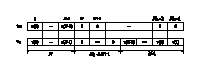
\includegraphics[keepaspectratio, scale=4]
					{parts/FourierAnalysis/imgs/FFT/arbitraryLengthFFT_to_powerOf2_FFT/u2,v2.eps}
					\caption{$u_2,v_2$の構造}
				\end{figure}
				このようにすると$u_2*v_2$の先頭$N$要素が$u*v$と一致する。
				\[ \text{FFT}(u_2*v_2) = \sqrt{N_2}\text{ FFT}(u_2) \text{ FFT}(v_2) \]
				より
				\[ \text{IFFT}(\sqrt{N_2}\text{ FFT}(u_2) \text{ FFT}(v_2)) \]
				により$u_2*v_2$を高速に計算し、結果の先頭$N$要素を切り出せば$u*v$を得る。
				得られた$u*v$の第$k$要素に$\frac{1}{\sqrt{N}} \exp \left(\pi i\frac{-k^2}{N}\right)$を掛ければ$x$のDFTが得られる。
				$v_2$のFFTや$\frac{1}{\sqrt{N}} \exp \left(\pi i\frac{-k^2}{N}\right) \;(k=0,1,\cdots,N-1)$は初回の計算結果を保存しておけば別の信号のDFTの計算で再利用できる。

	\part{Laplace変換}
	\chapter{複素指数関数入力に対する伝達関数の作用}
		\begin{shadebox}
			$A>0,\;\omega \in \realNumbers$とする。
			連続時間信号$f: \realNumbers \to \complexNumbers$を次のように定める。
			\[
				f(t) =
				\begin{cases}
					Ae^{i\omega t} & (t\geq 0) \\
					0 & (t<0)
				\end{cases}
			\]
			$H: s\in\complexNumbers \mapsto H(s) \in \complexNumbers$をproperで既約な有理関数とする。
			また、$H$の極の実部は全て負であるとする。
			伝達関数が$H(s)$である連続時間システムに信号$f$を入力した時の出力を$g$とすると、十分大きい$t$に対して
			$g(t) \sim H(i\omega)f(t)$となる。
		\end{shadebox}
		\begin{proof}
			\quad\par
			$N_\text{p}$を$H(s)$の分母多項式の相異なる零点の個数とし、それら零点を$p_0,\cdots,p_{N_\text{p}}$とする。
			零点$p_k$の次数を$N_{\text{p},k}$とし、$H(s)$の部分分数展開を
			\[ H(s) = c_0 + \sum_{k=1}^{N_\mathrm{p}} \sum_{l=1}^{N_{\mathrm{p},k}} \frac{c_{k,l}}{(s-p_k)^l} \]
			とする。
			ここに$c_0,c_{k,l}\;(k=1,\cdots,N_\mathrm{p},l=1,\cdots,N_{\mathrm{p},k})$は適当な複素数である。
			$f,g$のLaplace変換をそれぞれ$F,G$とすると$G(s) = H(s)F(s) = A H(s)/(s-i\omega)$である。
			これの部分分数展開に現れる、$1/(s-p_k)^l\;(k=1,\cdots,N_\mathrm{p},l=1,\cdots,N_{\mathrm{p},k})$に比例する項は逆Laplace変換すると$t^{l-1}e^{p_k t}$に比例する関数となり、$t\to\infty$で0に収束する。\hfill \rule{10cm}{0.4pt}(1)
			\par
			残りの項、すなわち$1/(s-i\omega)$に比例する項は$AH(i\omega)/(s-i\omega) = H(i\omega)F(s)$となる。
			以上より、十分大きい$t$に対して$g(t) \sim \ILPLC{H(i\omega)F(s)}(t) = H(i\omega)f(t)$となる。
		\end{proof}
		\section{系: 正弦波入力に対する伝達関数の作用}
			\begin{shadebox}
				$A>0,\;\omega \in \realNumbers$とする。
				連続時間信号$f_1,f_2: \realNumbers \to \realNumbers$を次のように定める。
				\[
					f_1(t) =
					\begin{cases}
						A\cos\omega t & (t\geq 0) \\
						0 & (t<0)
					\end{cases}
				\]
				\[
					f_2(t) =
					\begin{cases}
						A\sin\omega t & (t\geq 0) \\
						0 & (t<0)
					\end{cases}
				\]
				$H$を直前の定理と同じように定める。
				伝達関数が$H(s)$である連続時間\textcolor{red}{実}システムに信号$f_1,f_2$を入力した時の出力をそれぞれ$g_1,g_2$とすると、十分大きい$t$に対して
				\begin{align*}
					g_1(t) &\sim |H(i\omega)|\cos(\omega t + \Arg{H(i\omega)}) \\
					g_2(t) &\sim |H(i\omega)|\sin(\omega t + \Arg{H(i\omega)})
				\end{align*}
				となる。
			\end{shadebox}
			\begin{proof}
				\quad\par
				$f_1$について示す。
				$f_2$も同様に示せる。
				$f_1(t) = \Re{Ae^{i\omega t}}$であり、実数システムだから出力は$Ae^{i\omega t}$を入力したときの出力の実部と等しい。
				直前の定理の結果を用いて
				\[ g_1(t) = \Re{H(i\omega)Ae^{i\omega t}} = \Re{|H(i\omega)|e^{i\Arg{H(i\omega)}}Ae^{i\omega t}} = |H(i\omega)|\cos (\omega t + \Arg{H(i\omega)}) \]
			\end{proof}
			\begin{proof}
				(直接的な証明)
				\quad\par
				$f_1$について示す。
				$f_2$も同様に示せる。
				直前の定理の証明の(1)までは同じである。
				$f_1,g_1$のLaplace変換をそれぞれ$F_1,G_1$とすると
				\[ F_1(s) = \frac{As}{s^2+\omega^2} = \frac{A}{2}\left(\frac{1}{s+i\omega} + \frac{1}{s-i\omega}\right) \]
				であるから、$G_1(s) = H(s)F(s)$の部分分数展開のうち$1/(s+i\omega),\;1/(s-i\omega)$に比例する項を詳しく調べれば良い。
				$1/(s+i\omega)$の係数は
				\[ \left. G(s)X(s)(s+i\omega) \right|_{s\to-i\omega} = AG(-i\omega)/2\]
				となり、$1/(s-i\omega)$の係数は
				\[ \left. G(s)X(s)(s-i\omega) \right|_{s\to i\omega} = AG(i\omega)/2\]
				となる。
				よってこれらの項の和は
				\begin{align}
					&\quad \frac{AG(-i\omega)/2}{s+i\omega} + \frac{AG(i\omega)/2}{s-i\omega} = \frac{A}{2}\left(\frac{G(-i\omega)}{s+i\omega} + \frac{G(i\omega)}{s-i\omega}\right) \nonumber\\
					&= \frac{A}{2}\times\frac{1}{s^2+\omega^2}\left(G(-i\omega)(s-i\omega) + G(i\omega)(s+i\omega)\right) \nonumber\\
					&= \frac{As}{s^2+\omega^2}\times\frac{1}{2}(G(i\omega)+G(-i\omega)) + \frac{A\omega}{s^2+\omega^2}\times\frac{-1}{2i}(G(i\omega)-G(-i\omega))
				\end{align}
				$G(s)$は有理式なので$G(-i\omega) = \conj{G(i\omega)}$となることに注意して
				\[ \frac{1}{2}(G(i\omega)+G(-i\omega)) = |G(i\omega)|\frac{1}{2}\left(e^{i\Arg{G(i\omega)}} + e^{-i\Arg{G(i\omega)}}\right) = |G(i\omega)|\cos\Arg{G(i\omega)} \]
				同様に
				\[ \frac{-1}{2i}(G(i\omega)-G(-i\omega)) = -|G(i\omega)|\sin\Arg{G(i\omega)} \]
				以上より、
				\begin{align*}
					(1) &= |G(i\omega)|\left(\cos\Arg{G(i\omega)}\frac{As}{s^2+\omega^2} - \sin\Arg{G(i\omega)}\frac{A\omega}{s^2+\omega^2} \right) \\
					g(t) &\sim \ILPLC{(1)}(t) = |G(i\omega)|\left(\cos\Arg{G(i\omega)}\cos\omega t - \sin\Arg{G(i\omega)}\sin\omega t \right) \\
					&= |G(i\omega)|\cos\left(\omega t + \Arg{G(i\omega)}\right)
				\end{align*}
			\end{proof}
	\part{Z変換}
	\chapter{基礎理論}
		\section{最終値定理}
			\begin{shadebox}
				$X(z)\;(z\in\complexNumbers)$を離散時間信号$x(n)\;(n \in \integers,\;\forall n<0,x(n)=0)$のZ変換とする。
				$\lim_{n\to\infty} x(n)$が存在するとき次が成り立つ。
				\[ \lim_{z\to1}(z-1)F(z) = \lim_{n\to\infty} \]
				但し上式に於ける$\lim_{z\to1}$では$z$が実軸上で右側から1に近づくことを意味する。
			\end{shadebox}
			\begin{proof}
				\quad\par
				$\alpha = \lim_{n\to\infty} x(n)$とする。
				発想としては、十分大きい$N\in\naturalNumbers$に対して$\sum_{k=N}^\infty x(k)z^{-k} \sim \sum_{k=N}^\infty \alpha z^{-k} = \alpha z^{-N}\frac{z}{z-1}$となることを利用する。
				\par
				任意の$\varepsilon \in (0,1)$に対してある$N\in\naturalNumbers$が存在して$\forall n\geq N,\;|x(n)-\alpha|<\varepsilon$となる。
				\begin{align}
					\quad &\lim_{z\to1}(z-1)F(z) - \alpha = \lim_{z\to1}(z-1)z^N F(z) - \alpha \nonumber \\
					&= \lim_{z\to1}(z-1)z^N\left(\sum_{k=0}^{N-1} x(k)z^{-k} + \sum_{k=N}^\infty x(k)z^{-k}\right) - (z-1)z^N\sum_{k=N}^\infty \alpha z^{-k} \nonumber \\
					&= \lim_{z\to1}(z-1)z^N \sum_{k=N}^\infty (x(n) - \alpha)z^{-k} \quad \left(\sum_{k=0}^{N-1}\text{の項は極限で消える}\right) \\
					|(1)| &\leq \lim_{z\to1}(z-1)z^N \sum_{k=N}^\infty |x(n) - \alpha|z^{-k} < \lim_{z\to1}(z-1)z^N \sum_{k=N}^\infty \varepsilon z^{-k} = \varepsilon \nonumber
				\end{align}
			\end{proof}
		\section{複素指数関数入力に対する伝達関数の作用}
			\begin{shadebox}
				$A>0,\;\omega \in \realNumbers$とする。
				離散時間信号$x: \realNumbers \to \complexNumbers$を次のように定める。
				\[
					x(n) =
					\begin{cases}
						Ae^{i\Omega n} & (n\geq 0) \\
						0 & (n<0)
					\end{cases}
				\]
				$H: z\in\complexNumbers \mapsto H(z) \in \complexNumbers$を、$1/z$を変数とした有理式として既約であるような有理関数とする。
				また、$H$の極の絶対値は全て1未満であるとする。
				伝達関数が$H(z)$である離散時間システムに信号$x$を入力した時の出力を$y$とすると、十分大きい$n$に対して
				$y(n) \sim H(e^{i\Omega})x(n)$となる。
			\end{shadebox}
			\begin{proof}
				\quad\par
				$N_\text{p}$を$H(s)$の相異なる極の個数とし、それら極を$p_0,\cdots,p_{N_\text{p}}$とする。
				極$p_k$の次数を$N_{\text{p},k}$とし、$H(z)$の部分分数展開を
				\[ H(z) = c_0 + \sum_{k=1}^{N_\mathrm{p}} \sum_{l=1}^{N_{\mathrm{p},k}} \frac{c_{k,l}}{(1-p_kz^{-1})^l} \]
				とする。
				ここに$c_0,c_{k,l}\;(k=1,\cdots,N_\mathrm{p},l=1,\cdots,N_{\mathrm{p},k})$は適当な複素数である。
				$x,y$のZ変換をそれぞれ$X,Y$とすると$Y(z) = H(z)F(z) = A H(z)/(1-e^{i\Omega}z^{-1})$である。
				これの部分分数展開に現れる、$1/(1-p_k z^{-1})^l\;(k=1,\cdots,N_\mathrm{p},l=1,\cdots,N_{\mathrm{p},k})$に比例する項は逆Z変換すると$n$の多項式と公比$p_k$の等比級数の積となり、$n\to\infty$で0に収束する。
				(このことはZ変換の性質: 時間シフト$\mathcal{Z}[x(n+k)] = z^kX(z)$、およびZ領域微分$\mathcal{Z}[nx(n)] = -z\derivLong{\mathcal{Z}[x(n)]}{z}{}$を繰り返し用いることで分かる)
				\par
				残りの項、すなわち$1/(1-e^{i\Omega}z^{-1})$に比例する項は$AH(e^{i\Omega})/(1-e^{i\Omega}z^{-1}) = H(e^{i\Omega})X(z)$となる。
			\end{proof}
	\chapter{IIRフィルタの計算手順}
		\begin{figure}[H]
			\centering
			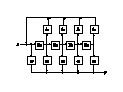
\includegraphics[keepaspectratio, scale=5]
			{parts/Z-transform/imgs/IIR-filter/calculationMethod/blockDiagram.eps}
			\caption{IIRフィルタのブロック図の例}
		\end{figure}
		上の例で示したIIRフィルタの出力は以下の手続きで計算できる(仕事で関わっていたデジタル無線機の信号処理部でそうやっていた)。
		\begin{enumerate}
			\item $D_1,\cdots D_4 \leftarrow 0$
			\item $n \leftarrow 0$
			\item $\alpha \leftarrow a_1D_1 + \cdots a_4D_4$
			\item $\beta \leftarrow b_1D_1 + \cdots b_4D_4$
			\item $\gamma \leftarrow x(n) + \beta$
			\item $y(n) \leftarrow \alpha + a_0\gamma$
			\item $D_4 \leftarrow D_3,\;D_3 \leftarrow D_2,\;D_2 \leftarrow D_1,\;D_1 \leftarrow \gamma$
			\item $n \leftarrow n+1$
			\item $n$が$x$の定義域の末尾に達しているなら終了。そうでないなら3に戻る。
		\end{enumerate}

	\begin{thebibliography}{99}
	\end{thebibliography}
\end{document}
